\section{Background from Non-Primary Tracks}\label{section:star_background_primary}
Reconstructed tracks matched to a~non-primary particle, so-called background tracks,  originate  mainly from the~following sources:
\begin{itemize}
	\item decays of short-lived primary particles with strange quark content (mostly $K^0$, $\Lambda^0$),
	\item photons from $\pi^0$ and $\eta$ decays which are converting to $e^+e^-$,
	\item hadronic interactions of particles with the beam-pipe or detector dead material.
\end{itemize} 

\begin{figure}[h!]
	\centering
	\begin{subfigure}{.45\textwidth}
		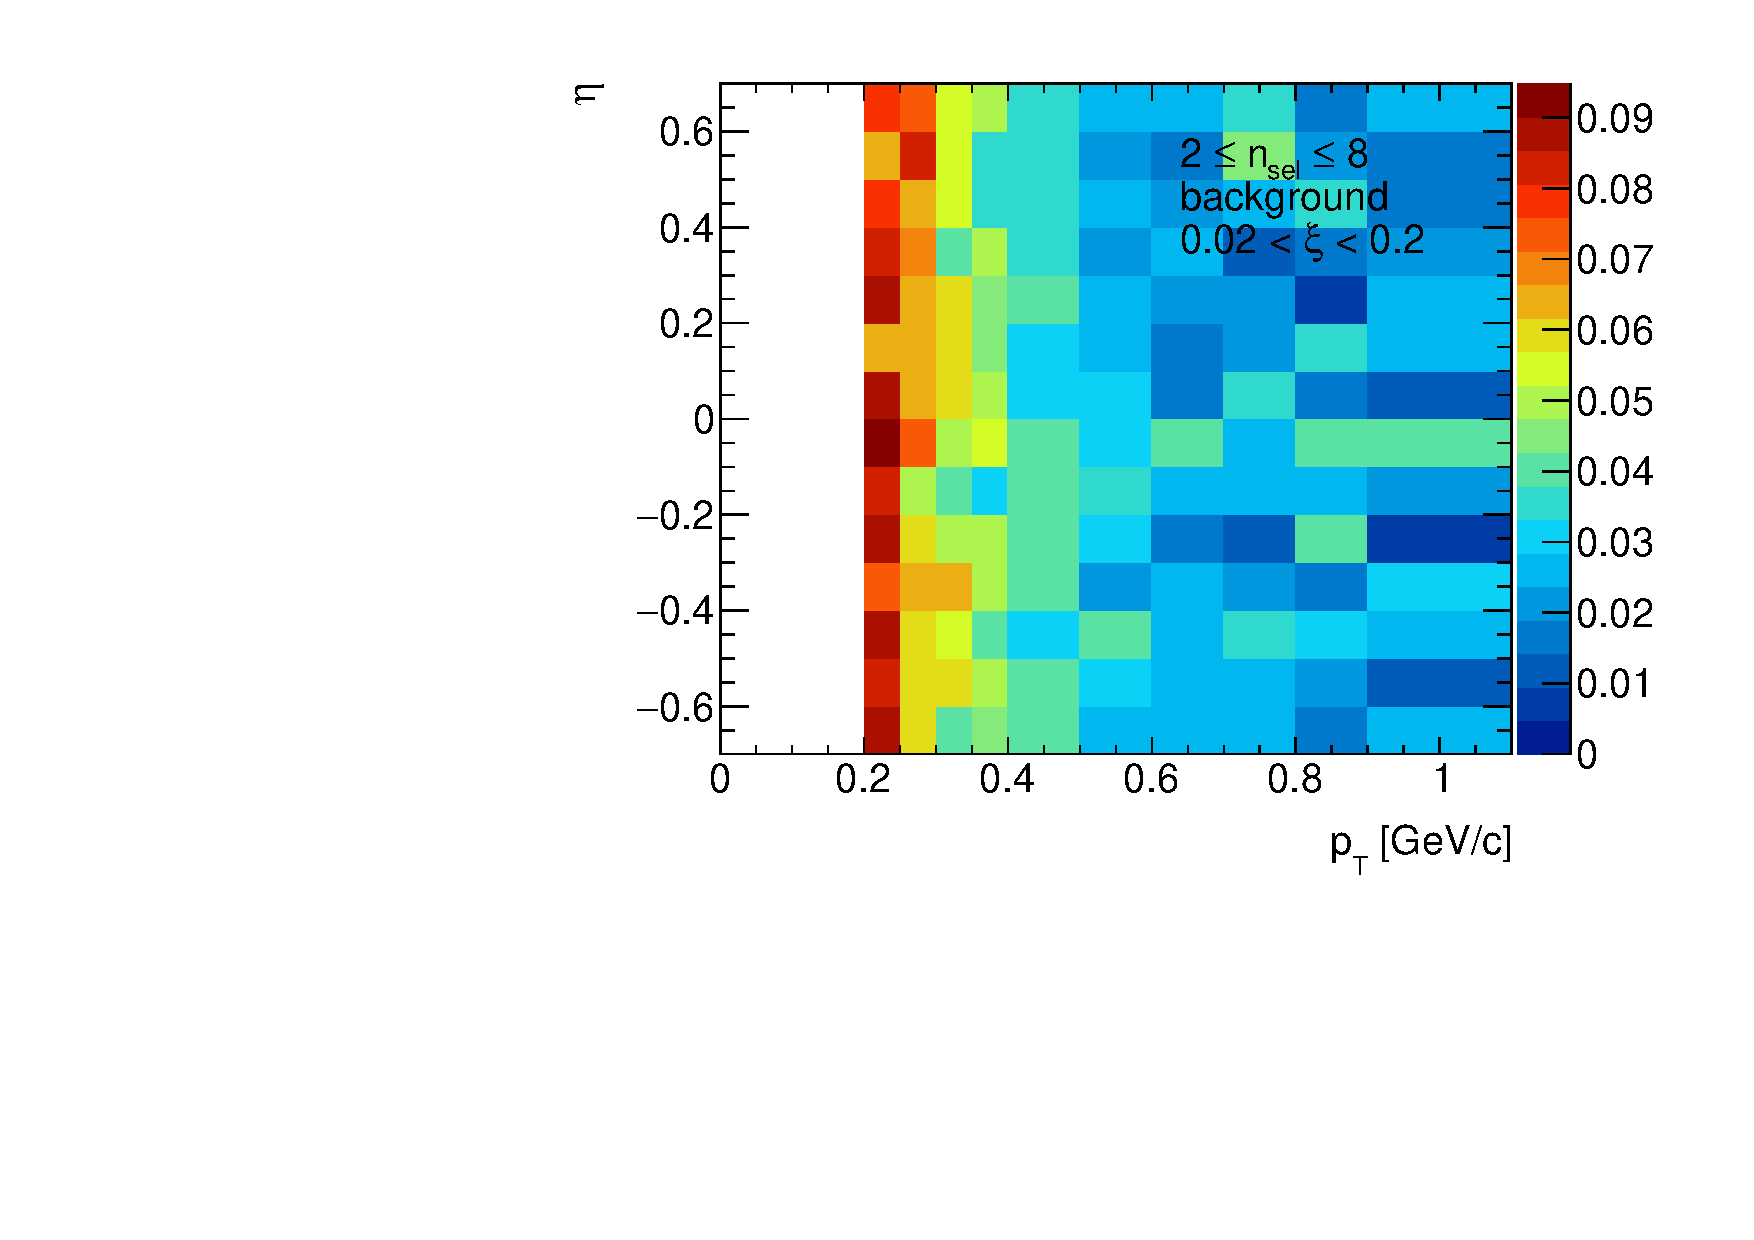
\includegraphics[width=\linewidth, page=1]{chapters/chrgSTAR/img/chargedBkg/bkg2D.pdf}
	\end{subfigure}
	\begin{subfigure}{.45\textwidth}
		\includegraphics[width=\linewidth, page=3]{chapters/chrgSTAR/img/chargedBkg/bkg2D.pdf}
	\end{subfigure}
\begin{comment}
	\begin{subfigure}{.45\textwidth}
		\includegraphics[width=\linewidth, page=4]{chapters/chrgSTAR/img/chargedBkg/bkg2D.pdf}
	\end{subfigure}
	\begin{subfigure}{.45\textwidth}
		\includegraphics[width=\linewidth, page=5]{chapters/chrgSTAR/img/chargedBkg/bkg2D.pdf}
	\end{subfigure}
\end{comment}
	\caption{(left) Distribution of fraction of selected tracks  associated with non-primary particles  in the~range $0.02<\xi<0.2$ and  (right) distribution of fraction of tracks which are not associated with true-level particles  in the~range $0.02<\xi<0.05$ as predicted by PYTHIA~8 4C (SaS) embedding.}
	\label{fig:bkg_fake_charged}
\end{figure}
There is also a contribution from fake tracks, i.e. tracks not associated with true-level particles, coming from out-of-time pile-up or  formed by a random combination of TPC hits. Figure~\ref{fig:bkg_fake_charged} shows the background $f_{\textrm{bkg}}\left(p_{\textrm{T}},\eta\right)$ and fake track $f_{\textrm{fake}}\left(p_{\textrm{T}},\eta\right)$ contribution to reconstructed tracks as a~function of $p_{\textrm{T}}$ and $\eta$. There were no differences observed in the~background contribution in different $\xi$ ranges, hence, all three $\xi$ ranges were merged for this study. The highest background fraction, which varies between $5-10\%$, was found to be at low $p_{\textrm{T}}$.  Due to too low statistics in PYTHIA~8 embedding \ac{MC}, the~shape of the~fake track contribution was assumed to be the~same in all three $\xi$ ranges. However, its normalization was calculated for each $\xi$ range separately with a ratio between the ranges of $1: 0.74: 1.11$.
The~change by $\pm100\%$ in fake track contribution was taken as a systematic uncertainty.


%\FloatBarrier
%background proton
\subsubsection{Proton Background}\label{section:star_background_proton}
Secondary particles can be created due to the interaction of particles with detector dead-material.
The proton sample contains background from such protons knocked out  from the~detector materials~\cite{STAR:spectra}. Most of these protons have large $\textrm{DCA}$ to the~primary vertex and are not associated with it. However, the~protons with small $\textrm{DCA}$  are included in the primary track sample. Antiprotons do not have knockout background, hence the~$\textrm{DCA}$ tail is almost absent in their $\textrm{DCA}$ distributions.

The fraction of knock-out background protons depends on a number of factors, including the~amount of detector material, analysis cuts and the $\xi$ of diffractive proton. While it is natural to calculate the fractions of primary and background protons in the~\ac{MC} sample, the \ac{MC} models do not necessarily predict the fraction of knock-out background protons without any bias. Hence,  data-driven methods should be used to calculate this type of background.

\begin{figure}[h!]
	\centering
	\begin{subfigure}{.49\textwidth}
		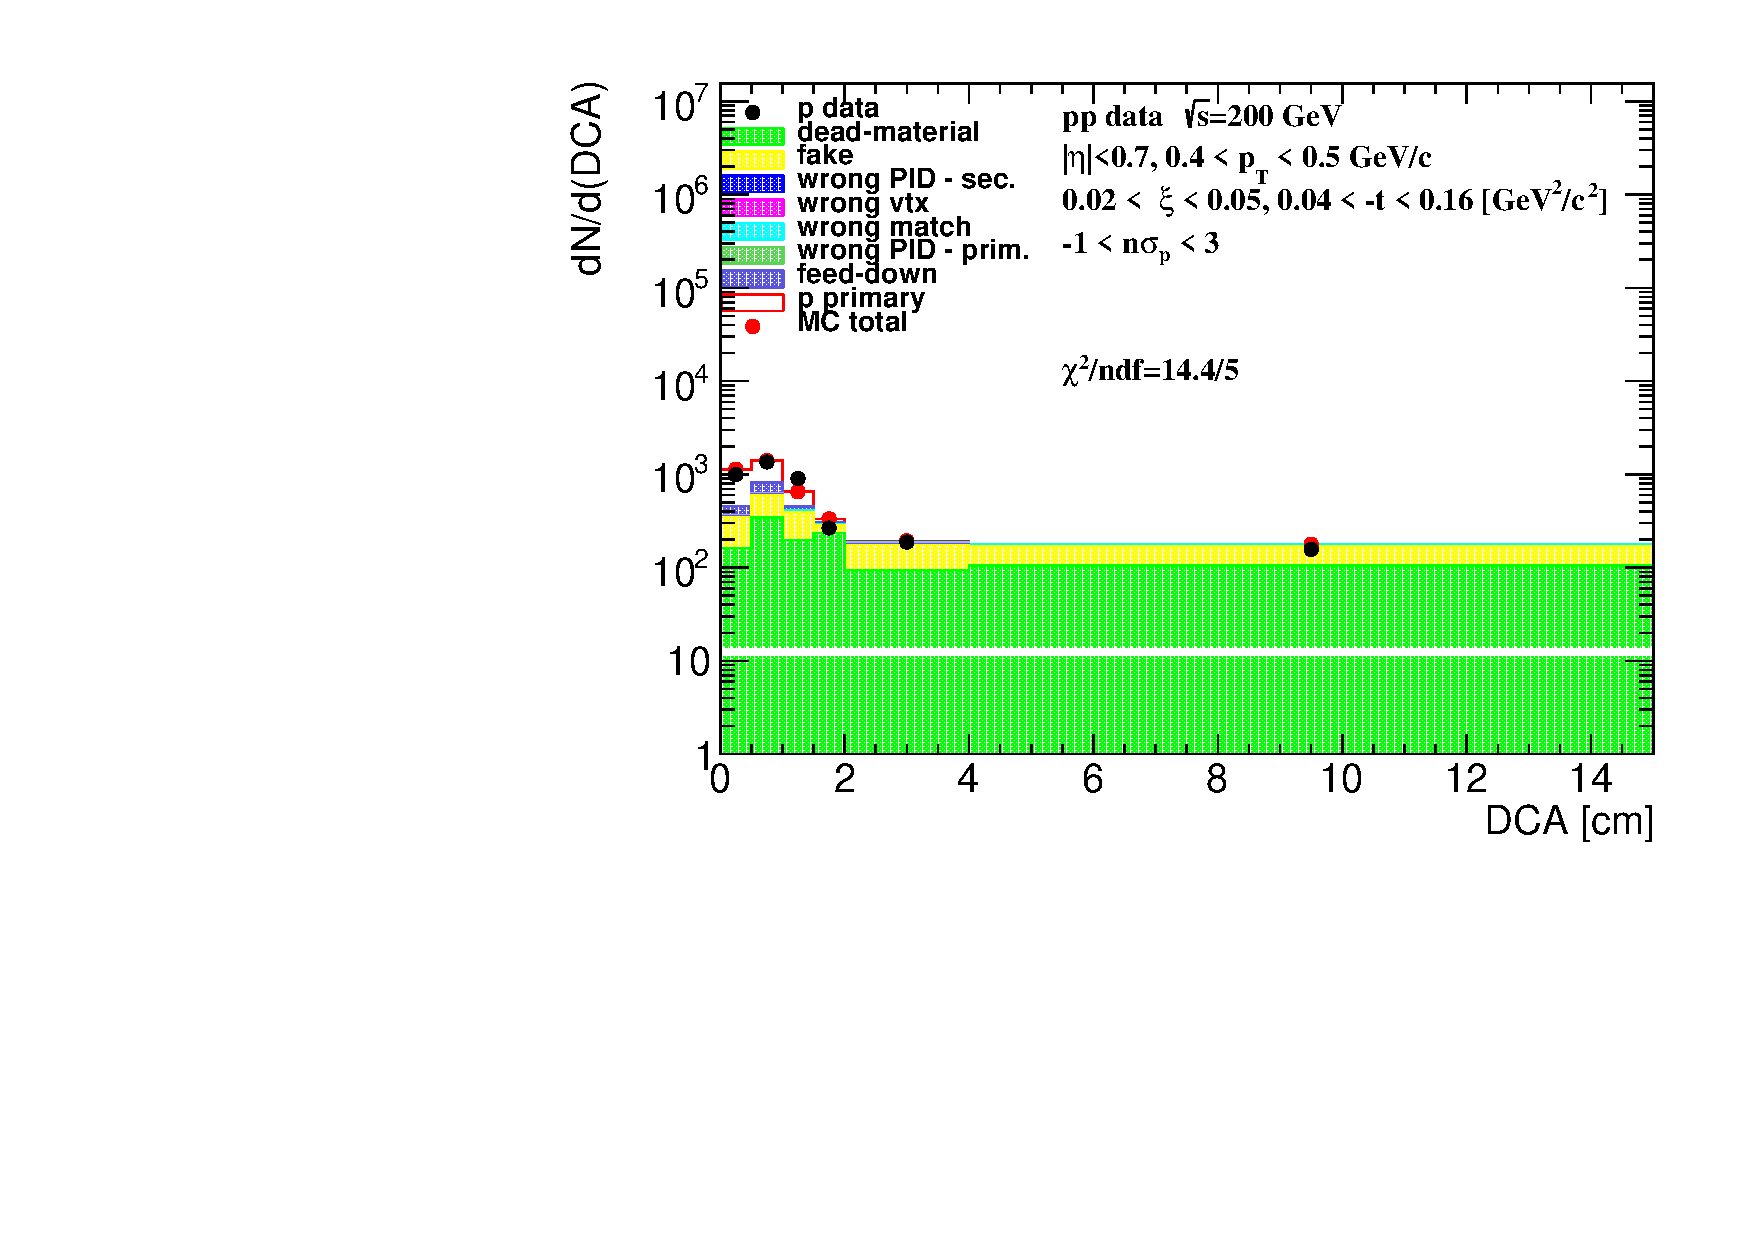
\includegraphics[width=\linewidth, page=1]{chapters/chrgSTAR/img/DCAproton/background_p_0.pdf}
	\end{subfigure}
	\begin{subfigure}{.49\textwidth}
		\includegraphics[width=\linewidth, page=2]{chapters/chrgSTAR/img/DCAproton/background_p_0.pdf}
	\end{subfigure}
	\begin{subfigure}{.49\textwidth}
		\includegraphics[width=\linewidth, page=3]{chapters/chrgSTAR/img/DCAproton/background_p_0.pdf}
	\end{subfigure}
	\begin{subfigure}{.49\textwidth}
		\includegraphics[width=\linewidth, page=4]{chapters/chrgSTAR/img/DCAproton/background_p_0.pdf}
	\end{subfigure}
	\caption{The $\textrm{DCA}$ distributions of protons for $0.4<p_T<0.5$~GeV/c shown for single range of $0.02<\xi<0.05$ (shown in log and linear scale in left and right column, respectively). The MC  contributions are shown after scaling the dead-material template  to the~tail of large $\textrm{DCA}$ values, $2<\textrm{DCA}<15$~cm. (top) Background enriched samples were used in the normalization procedure, whereas (bottom) the proton background was estimated from the nominal sample.}
	\label{fig:bkg_proton}
\end{figure}

In order to correct for the knock-out background protons, sample enriched in proton background  was used for background normalization, where $\textrm{DCA}_{xy}$, $\textrm{DCA}_z$ and $d_0$ cuts were abandoned. Additionally, at least one, instead of exactly one,  reconstructed vertex was allowed in this sample.  \Cref{fig:bkg_proton,fig:bkg_proton_bar} show the~$\textrm{DCA}$ distributions of protons and antiprotons, respectively, for  nominal (bottom) and background enriched (top) samples. The distributions for other $p_\textrm{T}$ and $\xi$ regions are shown in Appendix~\ref{appendix:DCA_proton}.
The protons and antiprotons are selected by a $dE/dx$ cut of $-1 < n\sigma_{p,\bar{p}} < 3$ where $n\sigma_{p,\bar{p}}$ is given by Eq.~\eqref{eq:nsigma}. In some $p_\textrm{T}$ regions, the~$dE/dx$ of (anti)protons and pions
starts to overlap, hence, the~asymmetric $n\sigma_{p,\bar{p}}$ cut was introduced in order to select as clean (anti)proton sample as possible.
The fraction of knock-out protons within the selected sample is determined via \ac{MC} template fits. The templates of reconstructed tracks with $dE/dx$ corresponding to the~proton and antiproton are obtained from PYTHIA~8 embedding \ac{MC} separately for:
\begin{itemize}
	\item primary (anti)protons,
	\item knock-out background protons (labeled as dead-material),
	\item fake tracks,
	\item secondary particles with $dE/dx$ of (anti)proton (labeled as wrong PID - sec.),
	\item tracks associated with primary (anti)protons, but with the reconstructed vertex  not matched to true-level primary vertex (labeled as wrong vtx),
	\item reconstructed track is partially matched to true-level particle (labeled as wrong match, track to true-level particle matching is described in~\cite{supplementaryNote}), i.e.  track and true-level particle have appropriate number of common hit points but the distance between true-level particle and track is too large, $\delta^2\left(\eta,\phi\right)>\left(0.15\right)^2$, thus, track is not considered as primary particle according to discussion in~\cite{supplementaryNote}, 
	\item primary particles with $dE/dx$ of (anti)proton (labeled as wrong PID - prim.),
	\item (anti)proton as a product of short-lived decays, mainly $\Lambda^0$ (labeled as feed-down).
\end{itemize}



First, the background enriched sample was analyzed  (Fig.~\ref{fig:bkg_proton}, top), where the template of knock-out background protons was normalized to the number of events in the fake-subtracted tail of the $\textrm{DCA}$ distribution, $2<\textrm{DCA}<15$~cm. Next the knock-out proton and fake background was subtracted from the $\textrm{DCA}$ distribution and the sum of other templates was normalized to the~number of events in the~signal region,  $\textrm{DCA}<1.5$~cm. 

\begin{figure}[h!]
	%\vspace{-1cm}
	\centering
	\begin{subfigure}{.49\textwidth}
		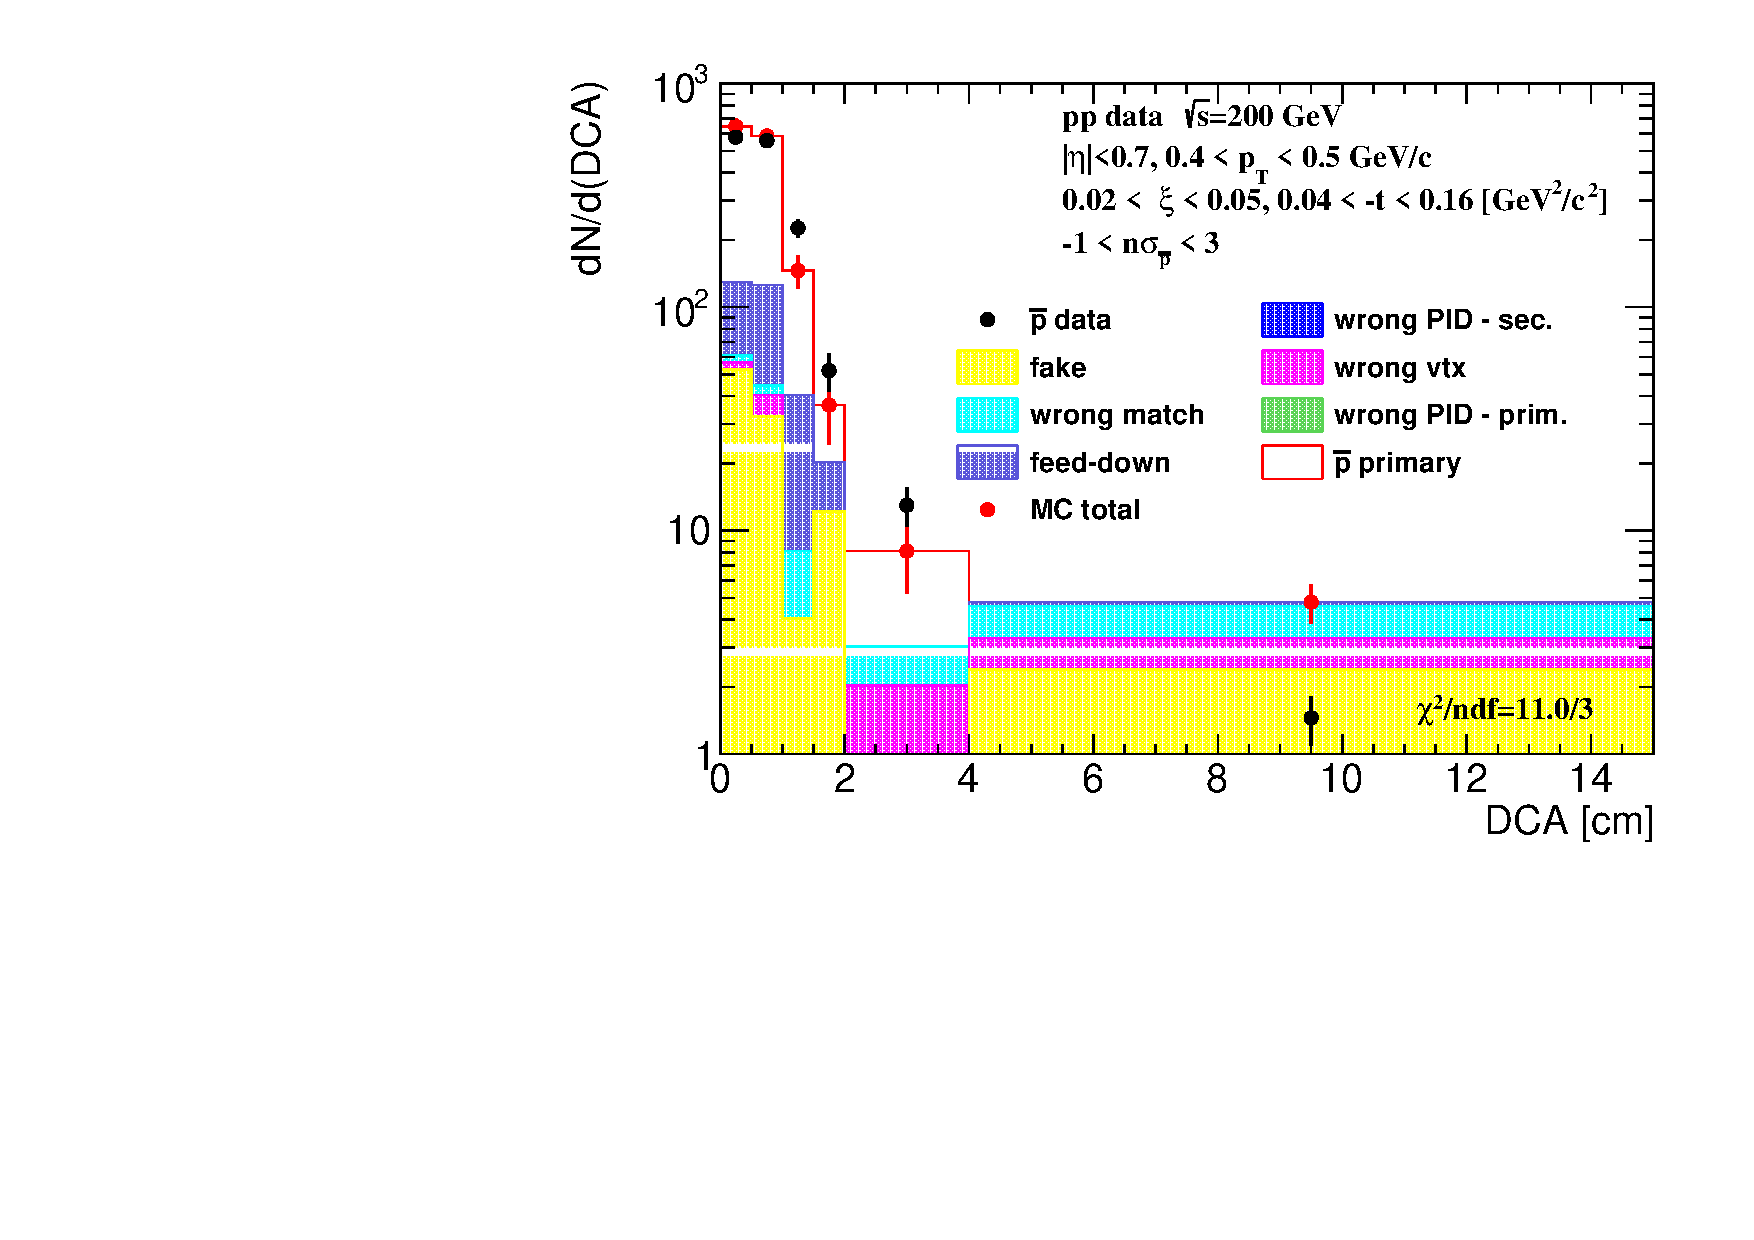
\includegraphics[width=\linewidth, page=1]{chapters/chrgSTAR/img/DCAproton/background_p_bar_0.pdf}
	\end{subfigure}
	\begin{subfigure}{.49\textwidth}
		\includegraphics[width=\linewidth, page=2]{chapters/chrgSTAR/img/DCAproton/background_p_bar_0.pdf}
	\end{subfigure}
	\begin{subfigure}{.49\textwidth}
		\includegraphics[width=\linewidth, page=3]{chapters/chrgSTAR/img/DCAproton/background_p_bar_0.pdf}
	\end{subfigure}
	\begin{subfigure}{.49\textwidth}
		\includegraphics[width=\linewidth, page=4]{chapters/chrgSTAR/img/DCAproton/background_p_bar_0.pdf}
	\end{subfigure}
	\caption{The $\textrm{DCA}$ distributions of antiprotons for $0.4<p_\textrm{T}<0.5$~GeV/c shown for one range of $0.02<\xi<0.05$ (log and linear scale in left and right column, respectively). The MC controbutions are shown as colour histograms. (top) Background enriched and (bottom) nominal samples were used.}
	\label{fig:bkg_proton_bar}
	%\vspace{-1cm}
\end{figure}

The fraction of the knock-out proton background in the signal region, $\textrm{DCA}<1.5$, was estimated from the nominal sample (Fig.~\ref{fig:bkg_proton}, bottom), where $\textrm{DCA}_{xy}$, $\textrm{DCA}_z$ and $d_0$ track cuts were applied and exactly one reconstructed vertex was required. The normalization of each MC contribution was kept the same as that estimated for the background enriched sample. Figure~\ref{fig:bkg_proton_fit} shows the knock-out proton background as a function of $p_\textrm{T}$ in three ranges of $\xi$. The following functional form was found to describe the
background protons:
\begin{equation}
f_{\textrm{bkg}}^{p}\left(p_\textrm{T}\right) = p_0\exp\left(p_1p_\textrm{T}\right)
\label{eq:protonBkgParametrization}
\end{equation}
where  $p_0$ and $p_1$ are  free parameters obtained from a~fit. 

The obtained fraction of knock-out background protons is approximately $20\%$ at $p_\textrm{T} = 0.45$ GeV/c
 and less than $10\%$ at $p_\textrm{T} = 1.0$~GeV/c.
 In PYTHIA~8 SD   predictions (also shown in~Fig.~\ref{fig:bkg_proton}), such fraction is much smaller  and equals to approximately $7\%$ at $p_\textrm{T} = 0.45$ GeV/c
 and about $5\%$ at $p_\textrm{T} = 1.0$~GeV/c. This may suggest that there are differences in the~amount of dead material in front of TPC  between data and simulation, which is consistent with the~studies presented in~\cite{supplementaryNote}.
 
 
 Figure~\ref{fig:bkg_proton_bar} shows the corresponding $\textrm{DCA}$ distributions with MC templates for antiprotons, where the background from knock-out particles is not present. Therefore, there was no need for any fit to be performed in this comparison. The MC templates  fairly well describe the $\textrm{DCA}$ distribution for both, protons, after tunning the~fraction of knock-out background to data, and antiprotons. %Additionally, there is a small $\left(<1\%\right)$ background  contribution, present for both particles, which also was taken into account and subtracted. It originates from reconstructed tracks which have the appropriate number of common hit points with true-level particle, but the~distance between them is too large, i.e. $\delta^2\left(\eta,\phi\right)>\left(0.15\right)^2$.
 

 \begin{figure}[h!]% \begin{wrapfigure}{r}{0.45\textwidth}
 	\centering
 	%\vspace{-20pt}
 	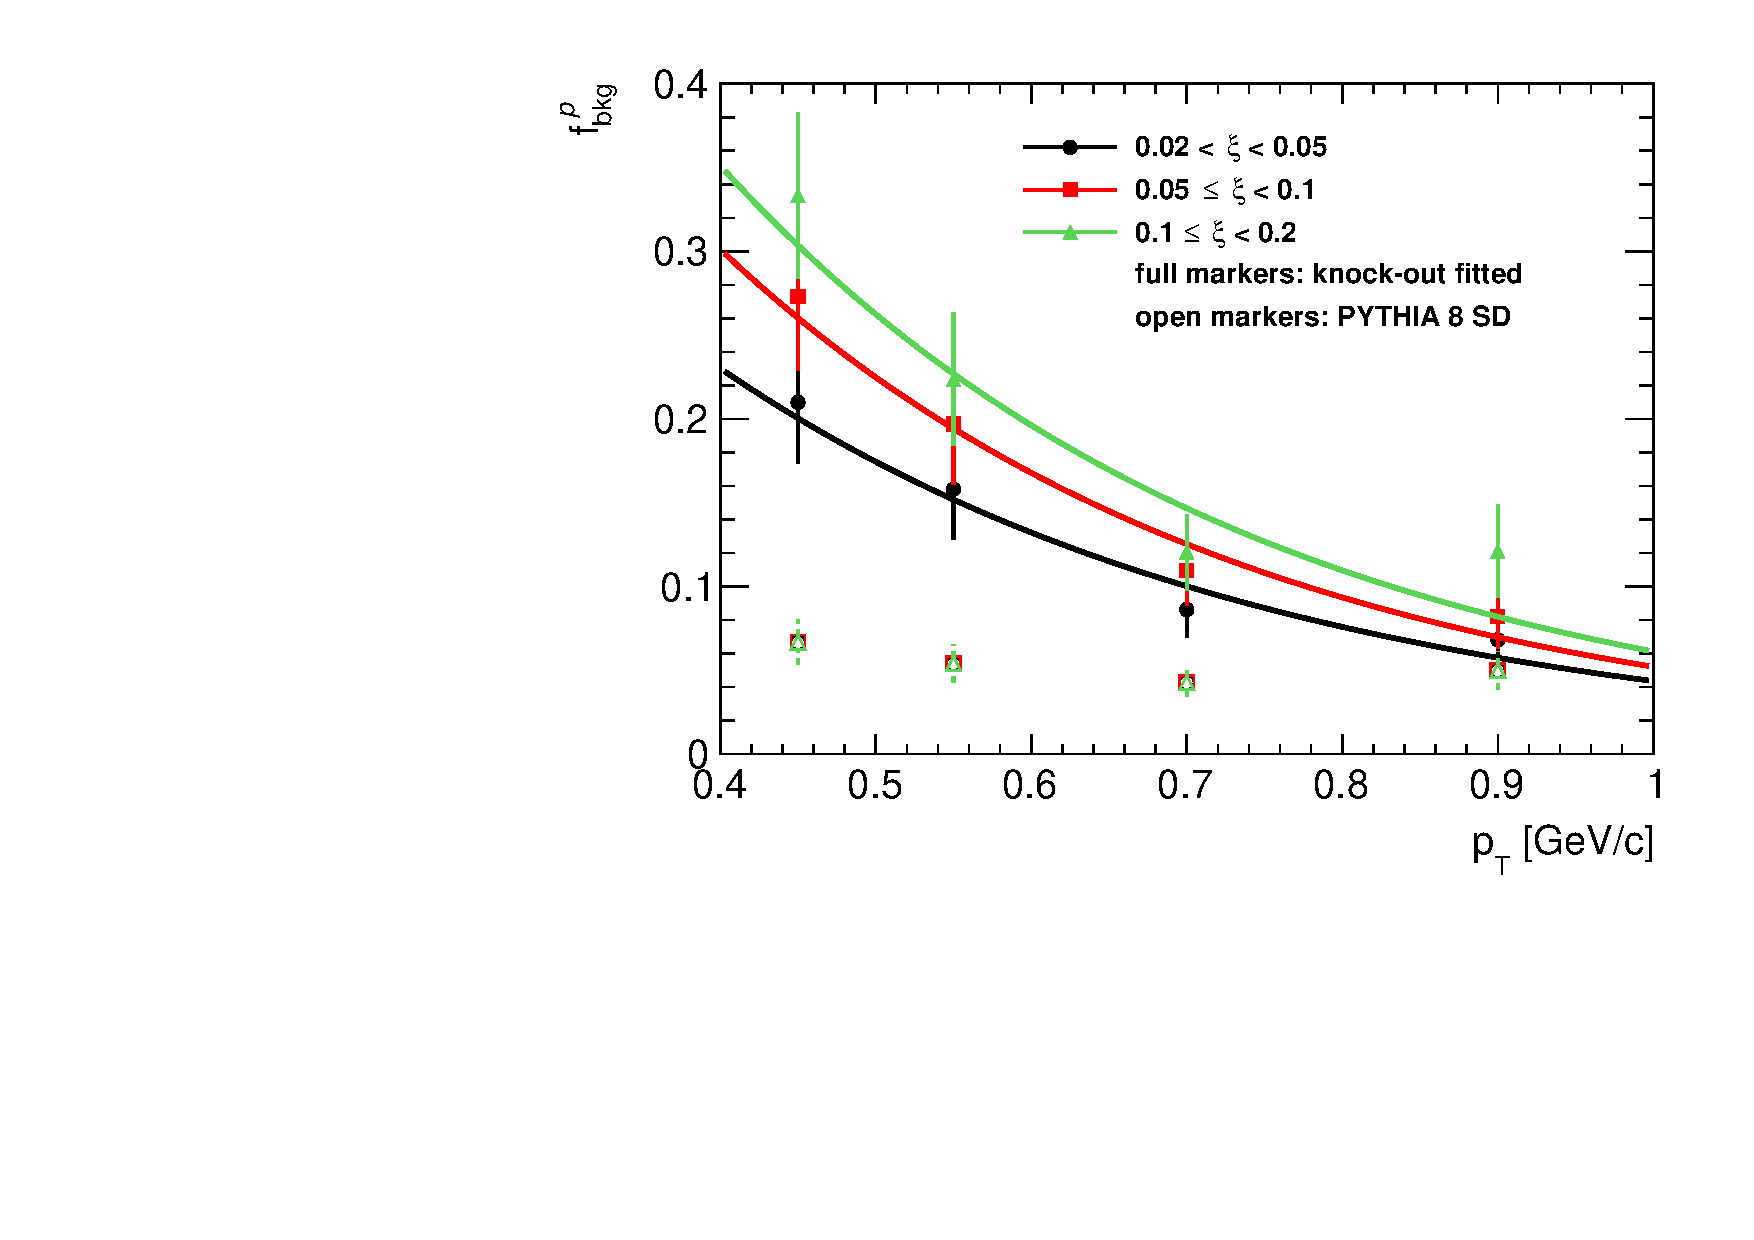
\includegraphics[width=0.8\linewidth, page=1]{chapters/chrgSTAR/img/DCAproton/bkg_p.pdf}
 	%\vspace{-20pt}
 	\caption{The fraction of knock-out proton background  as a function of $p_\textrm{T}$ in three ranges of $\xi$  with  fitted parametrizations. Full markers represent fitted knock-out background and open markers represent PYTHIA~8 SD predictions.}
 	%\vspace{-80pt}
 	\label{fig:bkg_proton_fit}
 \end{figure}

 
 \subsubsection{Systematic Uncertainty Related to Proton Background} 
The knock-out proton background estimation  introduces  systematic uncertainties. % which are added in quadrature. 
First, the normalization interval of the  knock-out   proton  background template in the background enriched sample was changed to $4<\textrm{DCA}<15$~cm. This introduced a relative systematic uncertainty of up to $30\%$ for $p_\textrm{T}\approx 0.9$~GeV/c. 

 \begin{figure}[h!]
 	\centering
 	\begin{subfigure}{.49\textwidth}
 		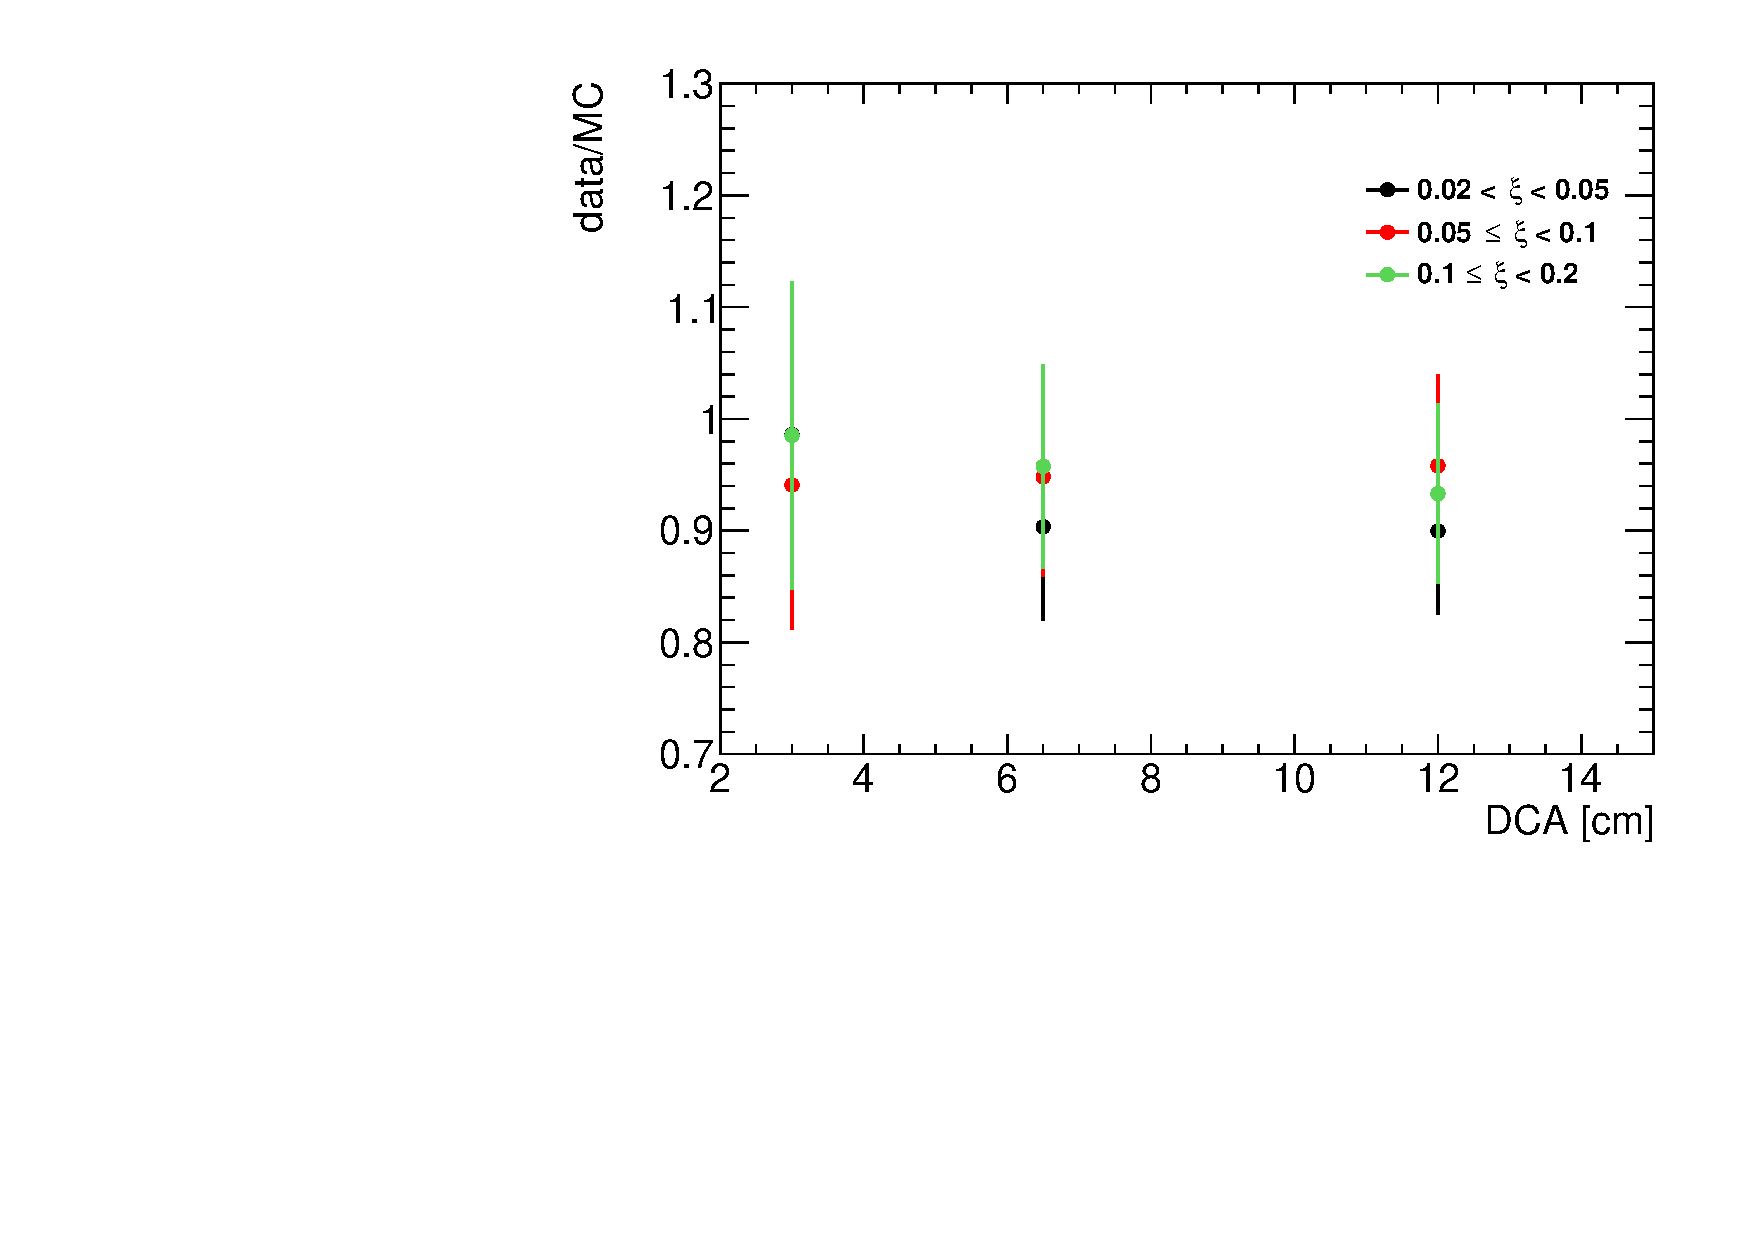
\includegraphics[width=\textwidth,page=1]{chapters/chrgSTAR/img/DCAproton/Ratio.pdf}
 	\end{subfigure}%\label{fig:protonBkgSystRatio}
 	\begin{subfigure}{.49\textwidth}
 		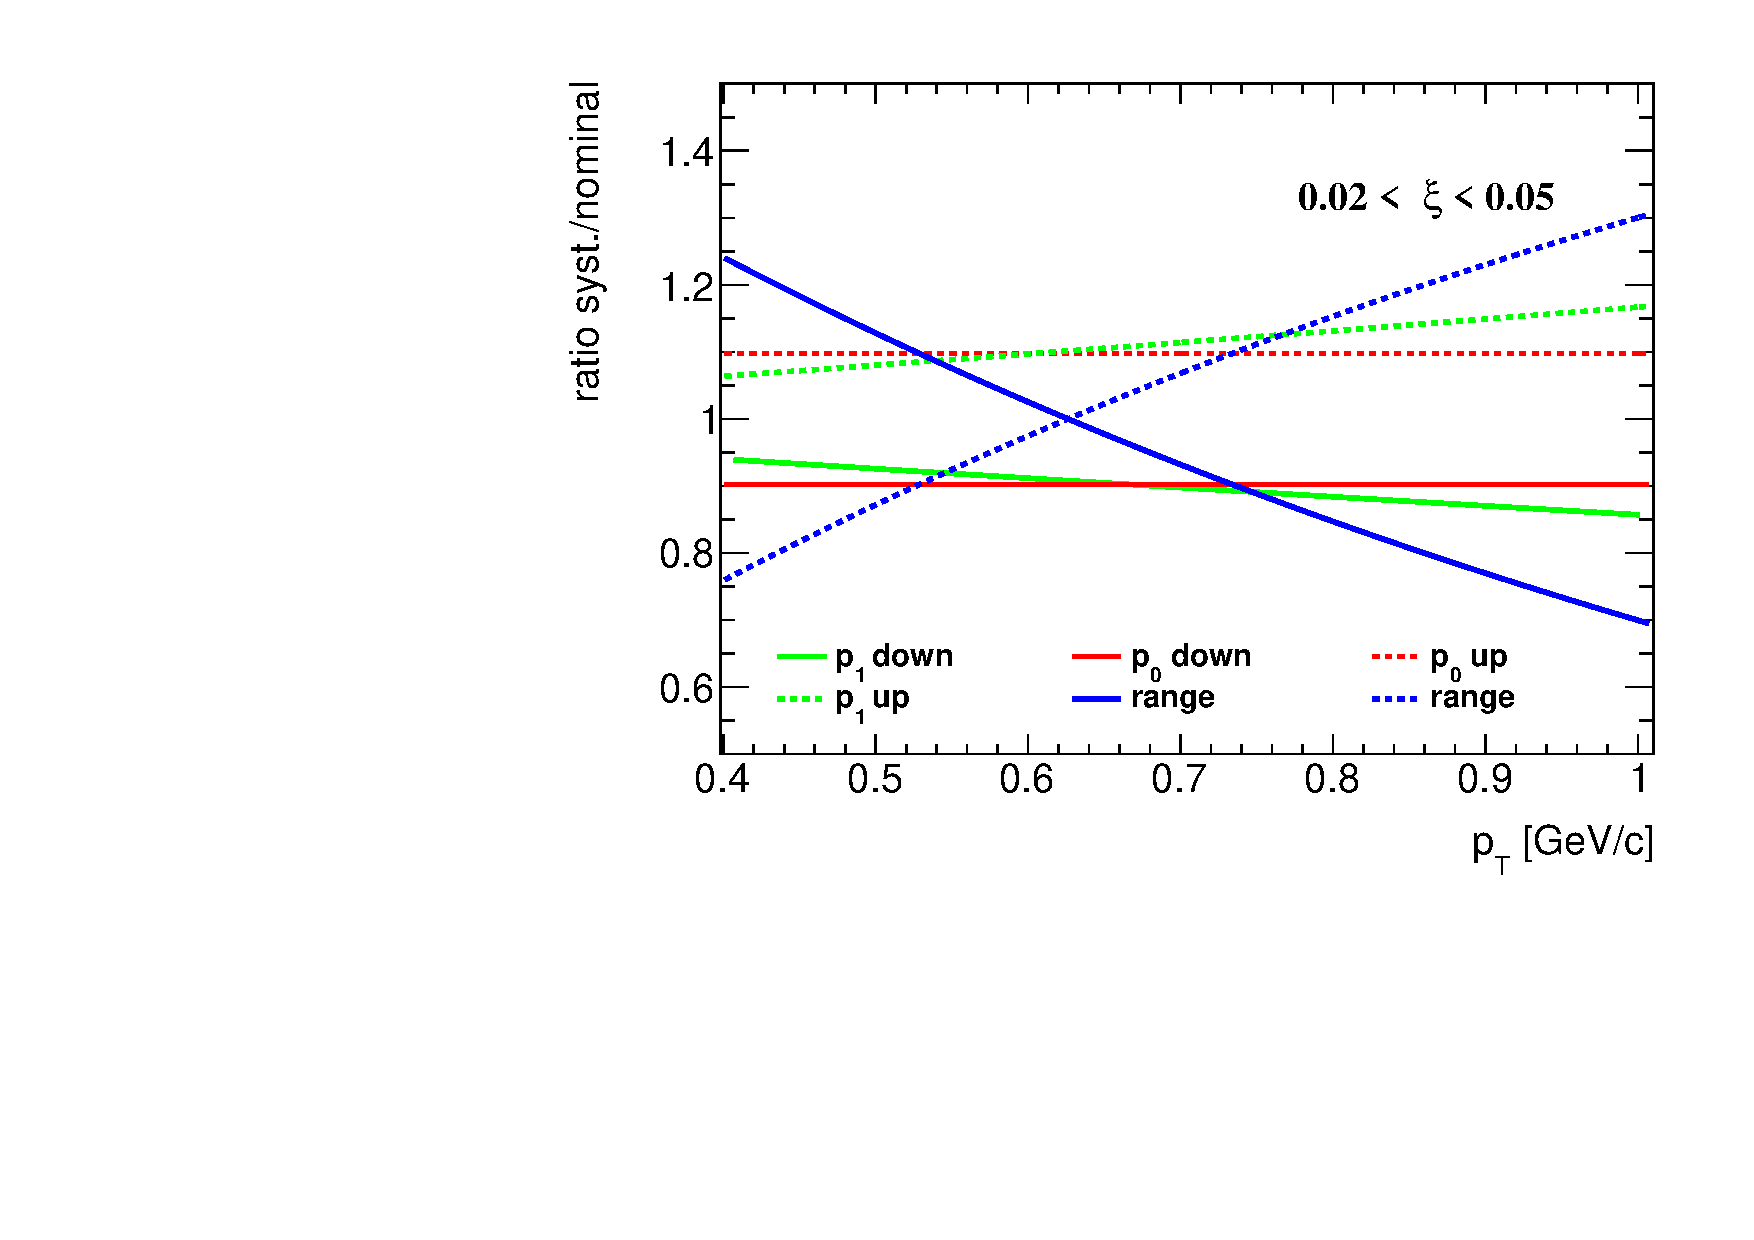
\includegraphics[width=\textwidth,page=1]{chapters/chrgSTAR/img/DCAproton/p_bkg.pdf}
 	\end{subfigure}
 	\begin{subfigure}{.49\textwidth}
 		\includegraphics[width=\textwidth,page=2]{chapters/chrgSTAR/img/DCAproton/p_bkg.pdf}
 	\end{subfigure}
 	\begin{subfigure}{.49\textwidth}
 		\includegraphics[width=\textwidth,page=3]{chapters/chrgSTAR/img/DCAproton/p_bkg.pdf}
 	\end{subfigure}
 	\caption{(top left) Data to MC ratio of  the  number of events in the background dominated region in three ranges of $\xi$ with fitted functional form given by Eq.~\eqref{eq:slopeBkgFit}. (top right and bottom) Components of the systematic uncertainty related to the  knock-out background protons contribution in three $\xi$ ranges. }
 	\label{fig:protonBkgSyst}
 	
 	\vspace{-1.5cm}
 \end{figure}

The  knock-out proton background contribution was  parameterized as  it is shown in  Eq.~\eqref{eq:protonBkgParametrization}. The systematic uncertainty related to the~parameterization procedure was estimated by varying the   parameters, $p_0$ and $p_1$, by their statistical uncertainties ($\pm1\sigma$).  As a result, a~relative systematic uncertainties of about $10\%$ were obtained.

Differences in the~shape of the~$\textrm{DCA}$ distribution between data and \ac{MC} can affect the~knock-out proton background estimation procedure. Figure~\ref{fig:protonBkgSyst} (top left) shows the data to MC ratio of  the  number of events in the background dominated region, $2<\textrm{DCA}<15$~cm. 
Since this region is used to estimate background normalization, and the shape of the $\textrm{DCA}$ distribution in the data differs from that observed in the simulation, the predicted background in the~$\textrm{DCA} <1.5$~cm region can change. Thus, the following functional form was used to estimate the slope between data and MC:
\begin{equation}
\frac{\textrm{data}}{\textrm{MC}}\left(\textrm{DCA}\right) = A(\textrm{DCA}-8.5)+B
\label{eq:slopeBkgFit}
\end{equation}
where $A$ (slope) and  $B$ are fit free parameters. Differences in slope between data and \ac{MC} were used to estimate how many
more background tracks would fit into the signal region and a systematic uncertainty, which varies up to $5\%$ for $0.02< \xi<0.05$, was introduced. 




All above components of the systematic uncertainty related to the knock-out proton background,  shown in Fig.~\ref{fig:protonBkgSyst}, are added in quadrature.
Those related to the~fit range and the~shape of the~proton background are symmetrized. Figure~\ref{fig:protonBkgSystSummary} shows the~fraction of knock-out proton background in three ranges of $\xi$ and the~total systematic uncertainty related to it.

\begin{figure}[h!]
	\centering
	\begin{subfigure}{.49\textwidth}
		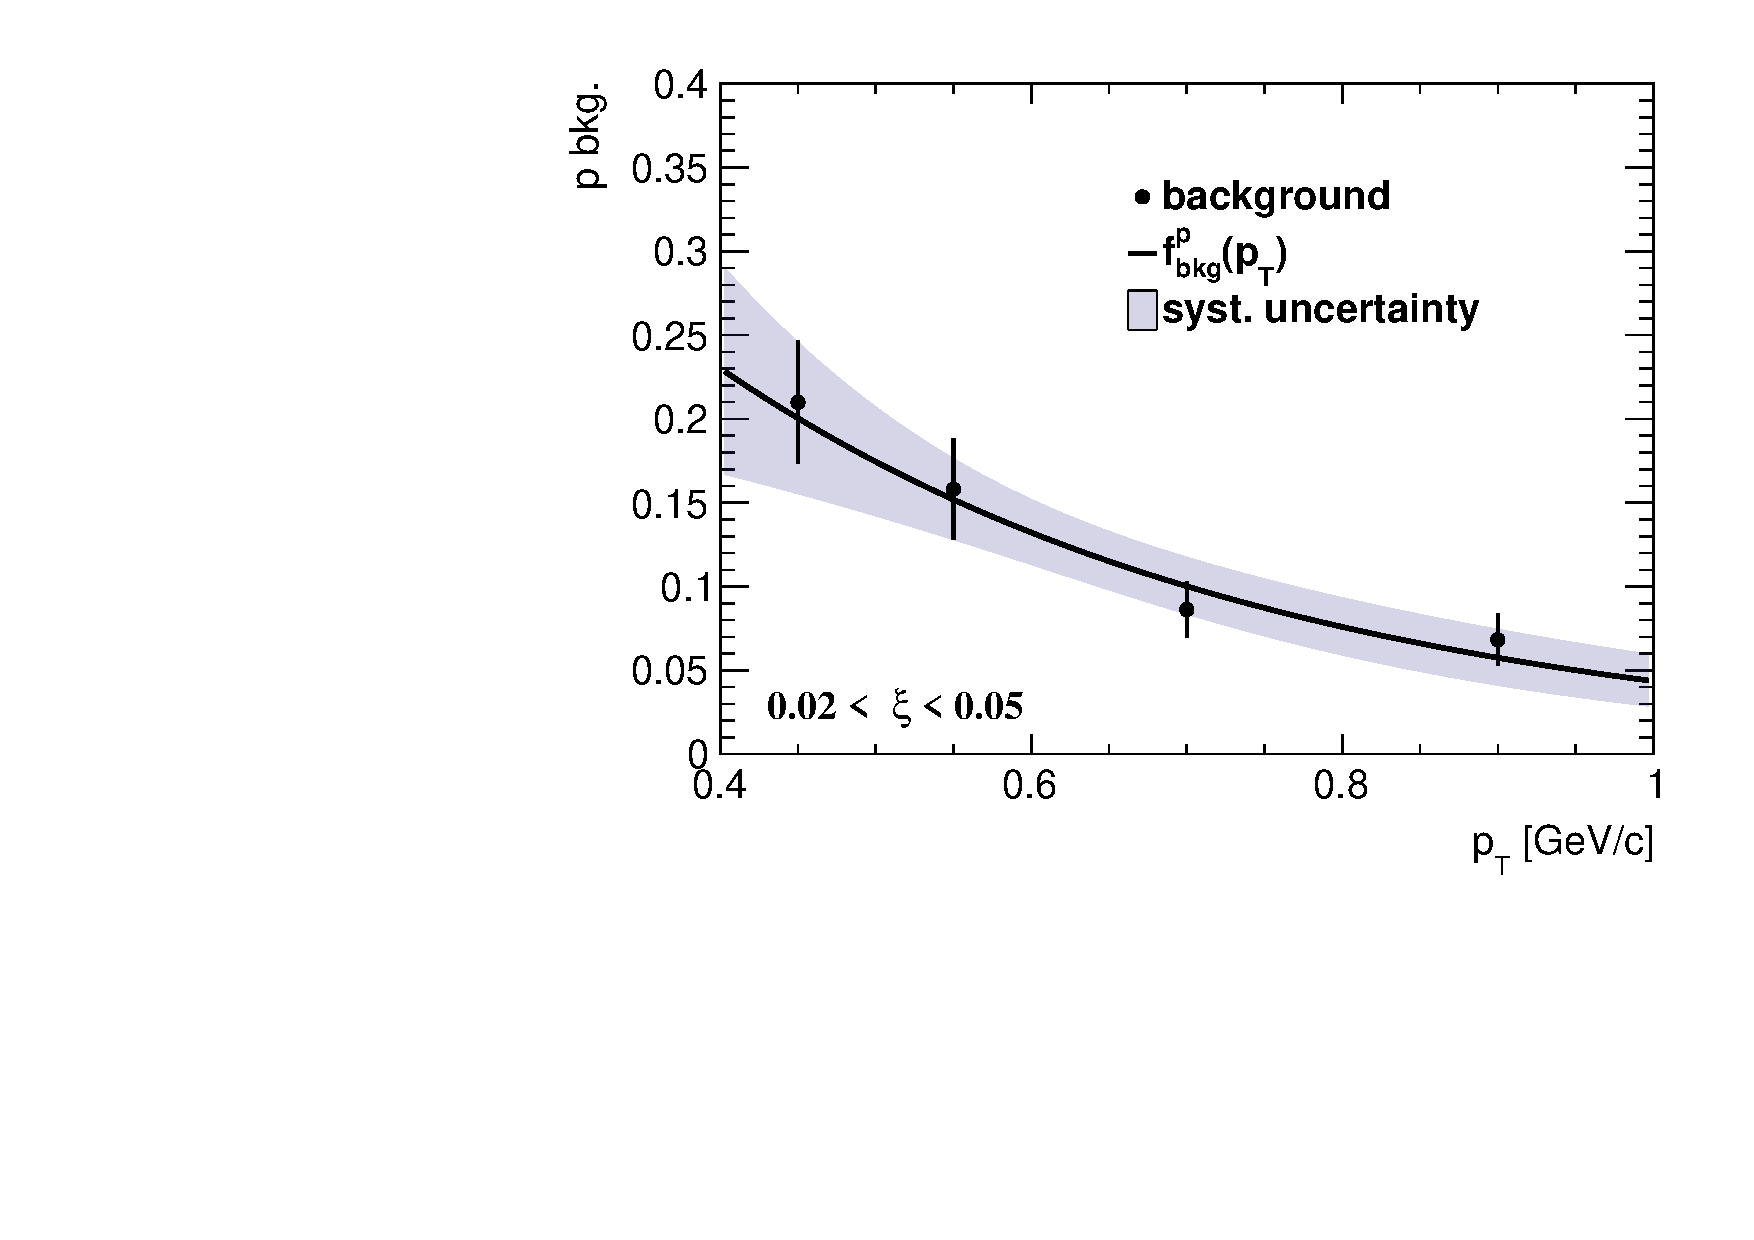
\includegraphics[width=\textwidth,page=1]{chapters/chrgSTAR/img/DCAproton/p_bkg_summary.pdf}
	\end{subfigure}%\label{fig:protonBkgSystRatio}
	\begin{subfigure}{.49\textwidth}
		\includegraphics[width=\textwidth,page=2]{chapters/chrgSTAR/img/DCAproton/p_bkg_summary.pdf}
	\end{subfigure}
	\begin{subfigure}{.49\textwidth}
		\includegraphics[width=\textwidth,page=3]{chapters/chrgSTAR/img/DCAproton/p_bkg_summary.pdf}
	\end{subfigure}
	\begin{minipage}{.49\textwidth}
			\caption{The fraction of knock-out proton background  as a function of $p_\textrm{T}$   with  fitted parametrizations in three ranges of $\xi$: (top left) $0.02 < \xi < 0.05$, (top right) $0.05<\xi<0.1$ and (bottom) $0.1<\xi<0.2$. Gray bands represent total systematic uncertainties.}
			\label{fig:protonBkgSystSummary}
	\end{minipage}
\end{figure}


 
 \FloatBarrier
%background pion
\subsubsection{Pion Background}\label{section:star_background_pion}
The pion spectra are corrected for weak decays (mainly of $K^0_S$ and $\Lambda^0$), muon contribution and background from the   detector dead-material interactions. The pion decay muons can be identified as pions due to the similar masses. These contributions are obtained from PYTHIA~8 \ac{SD}. Figure~\ref{fig:bkg_pion} shows the background contribution to the pion spectra as a function of $p_\textrm{T}$ in three ranges of $\xi$, separately for $\pi^-$ and $\pi^+$.  Since there were   negligible differences  observed between these  three ranges of $\xi$, the background contribution was averaged over $\xi$. The following parametrization was found to describe it:
\begin{equation}
f_{\textrm{bkg}}^{\pi}\left(p_\textrm{T}\right)=a_0\exp(a_1p_\textrm{T})+a_2p_\textrm{T}^2+a_3p_\textrm{T}
\end{equation}
where $a_i$, $i=0,\dots, 3$ are free paramaters of the fitted function. 

The pion background contribution varies between $5\%$ at low-$p_\textrm{T}$  ($p_\textrm{T}=0.25$~GeV/c) and about $1\%$ at $p_\textrm{T}=1.0$~GeV/c for both negatively and positively charged pions. In addition, the~background was calculated from EPOS SD+SD$^\prime$ for the~full range of $\xi$. The~differences between PYTHIA~8 and EPOS are up to $1\%$ for $\pi^-$. 
\begin{figure}[htpb]
	\centering
	\begin{subfigure}{.49\textwidth}
		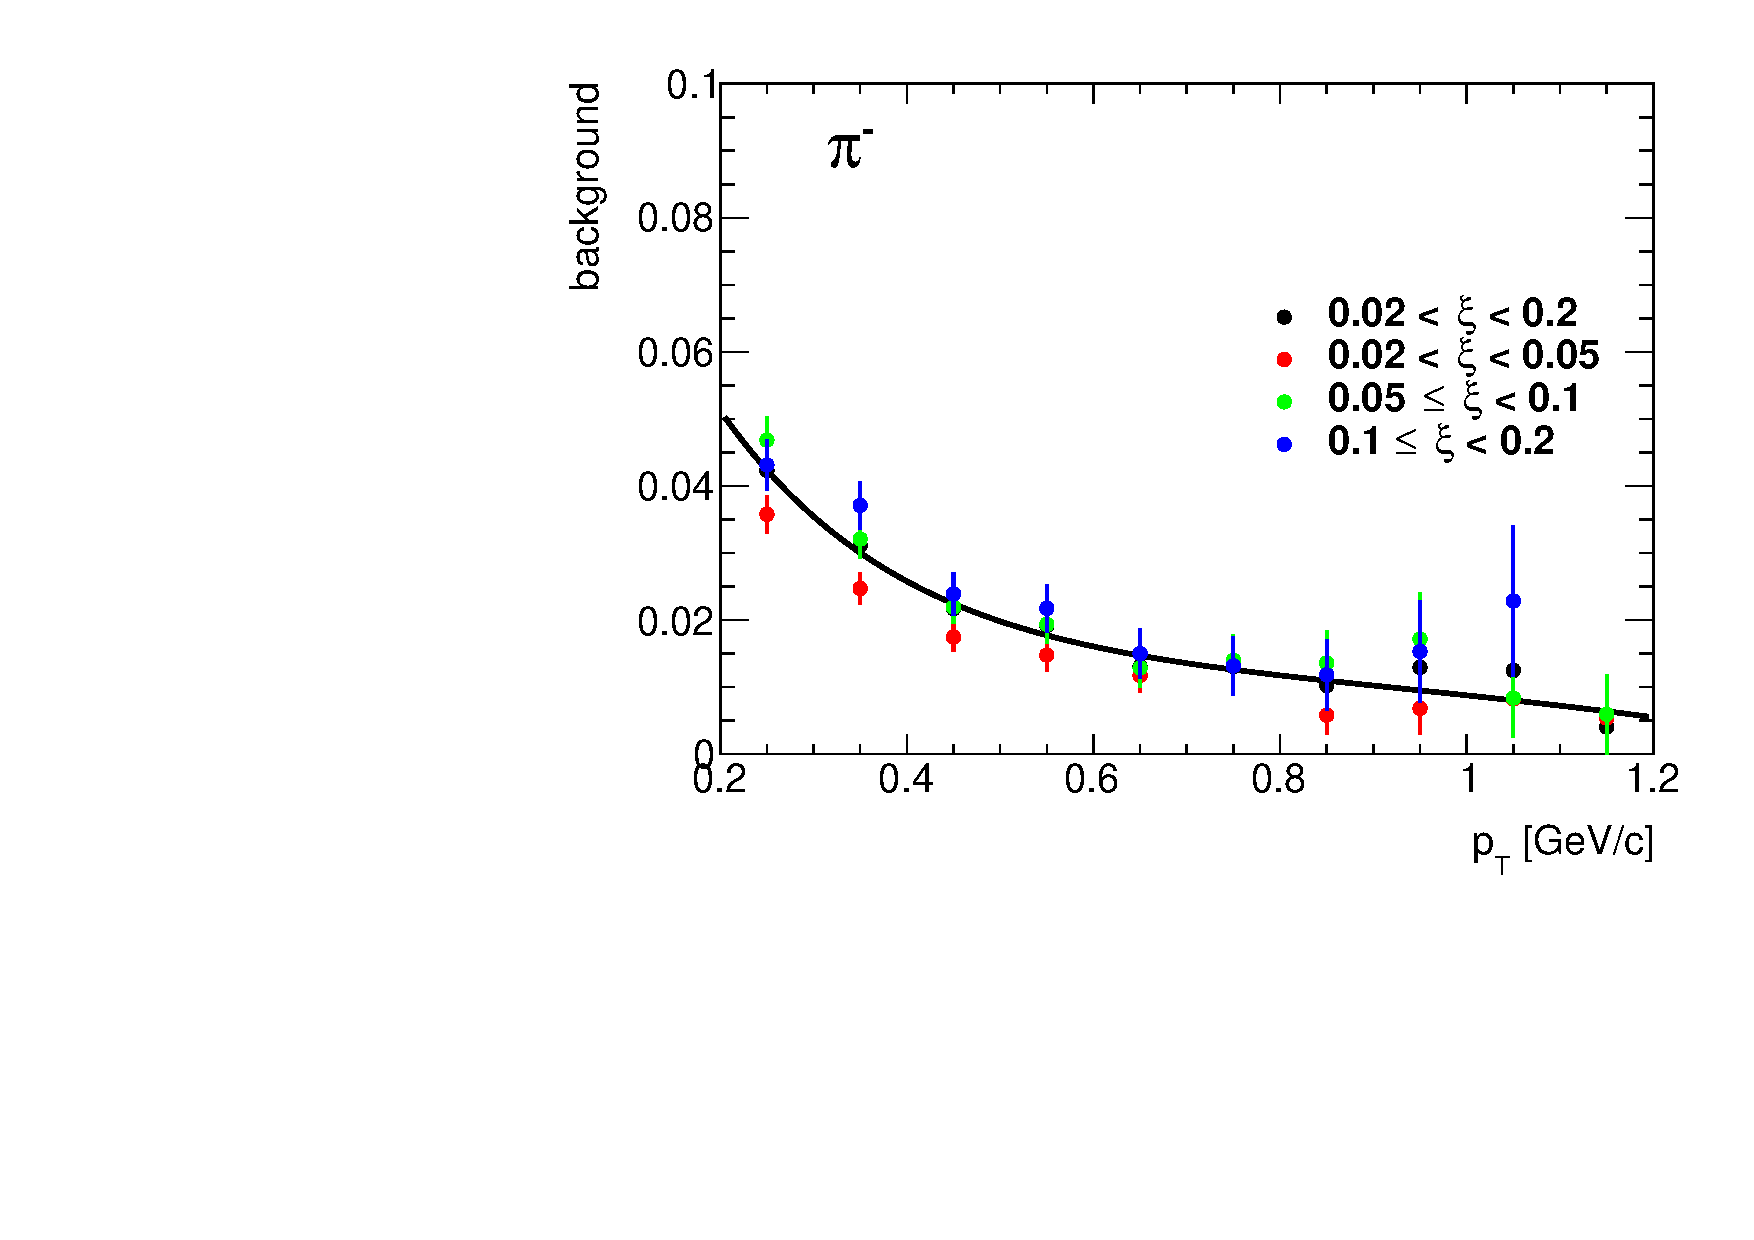
\includegraphics[width=\linewidth, page=1]{chapters/chrgSTAR/img/chargedBkg/bkg0max.pdf}
	\end{subfigure}
	\begin{subfigure}{.49\textwidth}
		\includegraphics[width=\linewidth, page=2]{chapters/chrgSTAR/img/chargedBkg/bkg0max.pdf}
	\end{subfigure}
	\caption{Pion background fraction as a function of $p_\textrm{T}$ calculated from PYTHIA~8 and shown separately for  (left) negatively  and (right)  positively charged pions in three ranges of $\xi$: (red) $0.02<\xi<0.05$,  (green) $0.05<\xi<0.1$, (blue) $0.1<\xi<0.2$.  (full black points) The pion background averaged over three ranges of $\xi$ with fitted parametrization is also shown. Open black points represent EPOS predictions for the full $\xi$ range.}
	\label{fig:bkg_pion}
\end{figure}

\FloatBarrier
